\subsubsection{Instrument Signature Removal}
\label{ssec:isr}
The first step in processing \gls{LSSTComCam} images is to correct for the effects introduced by the telescope and detector.
Each sensor and its readout amplifiers can vary slightly in performance, causing images of even a uniformly illuminated focal plane to exhibit discontinuities and shifts due to detector effects.
The \gls{ISR} pipeline aims to recover the original astrophysical signal as best as possible and produce science-ready single-epoch images for source detection and measurement (see \citealt{SITCOMTN-086,2025JATIS..11a1209P} for a detailed description of the \gls{ISR} procedures).

\figref{fig:isr_signal_chain} illustrates the model of detector components and readout electronics and their impact on the signal, tracing the process from photons incident on the detector surface to the final quantized values\footnote{The images written to disk by the camera have values that are integers., which come from the ADC converting an analog voltage.} recorded in the image files.
The \gls{ISR} \gls{pipeline} essentially ``works backward'' through the signal chain, correcting the integer analog-to-digital units (ADU) raw camera output back to a floating-point number of photoelectrons created in the silicon.
The physical detector, shown on the left in  \figref{fig:isr_signal_chain}, is the source of effects that arise from the silicon itself, such as the dark current and the brighter-fatter effect \citep{doi:10.1088/1538-3873/aab820,2024PASP..136d5003B}.
After the integration time has elapsed, the charge is shifted  to the serial register and read out, which can introduce charge transfer inefficiencies and a clock-injected offset level.
The signals for all amplifiers are transferred via cables to the \gls{REB}, during which crosstalk between the amplifiers may occur.
The \gls{ASPIC} on the \gls{REB} converts the analog signal from the detector into a digital signal, adding both quantization and a bias level to the image.
Although the signal chain is designed to be stable and linear, the presence of numerous sources of non-linearity indicates otherwise.
\begin{figure}[htb]
  \centering
  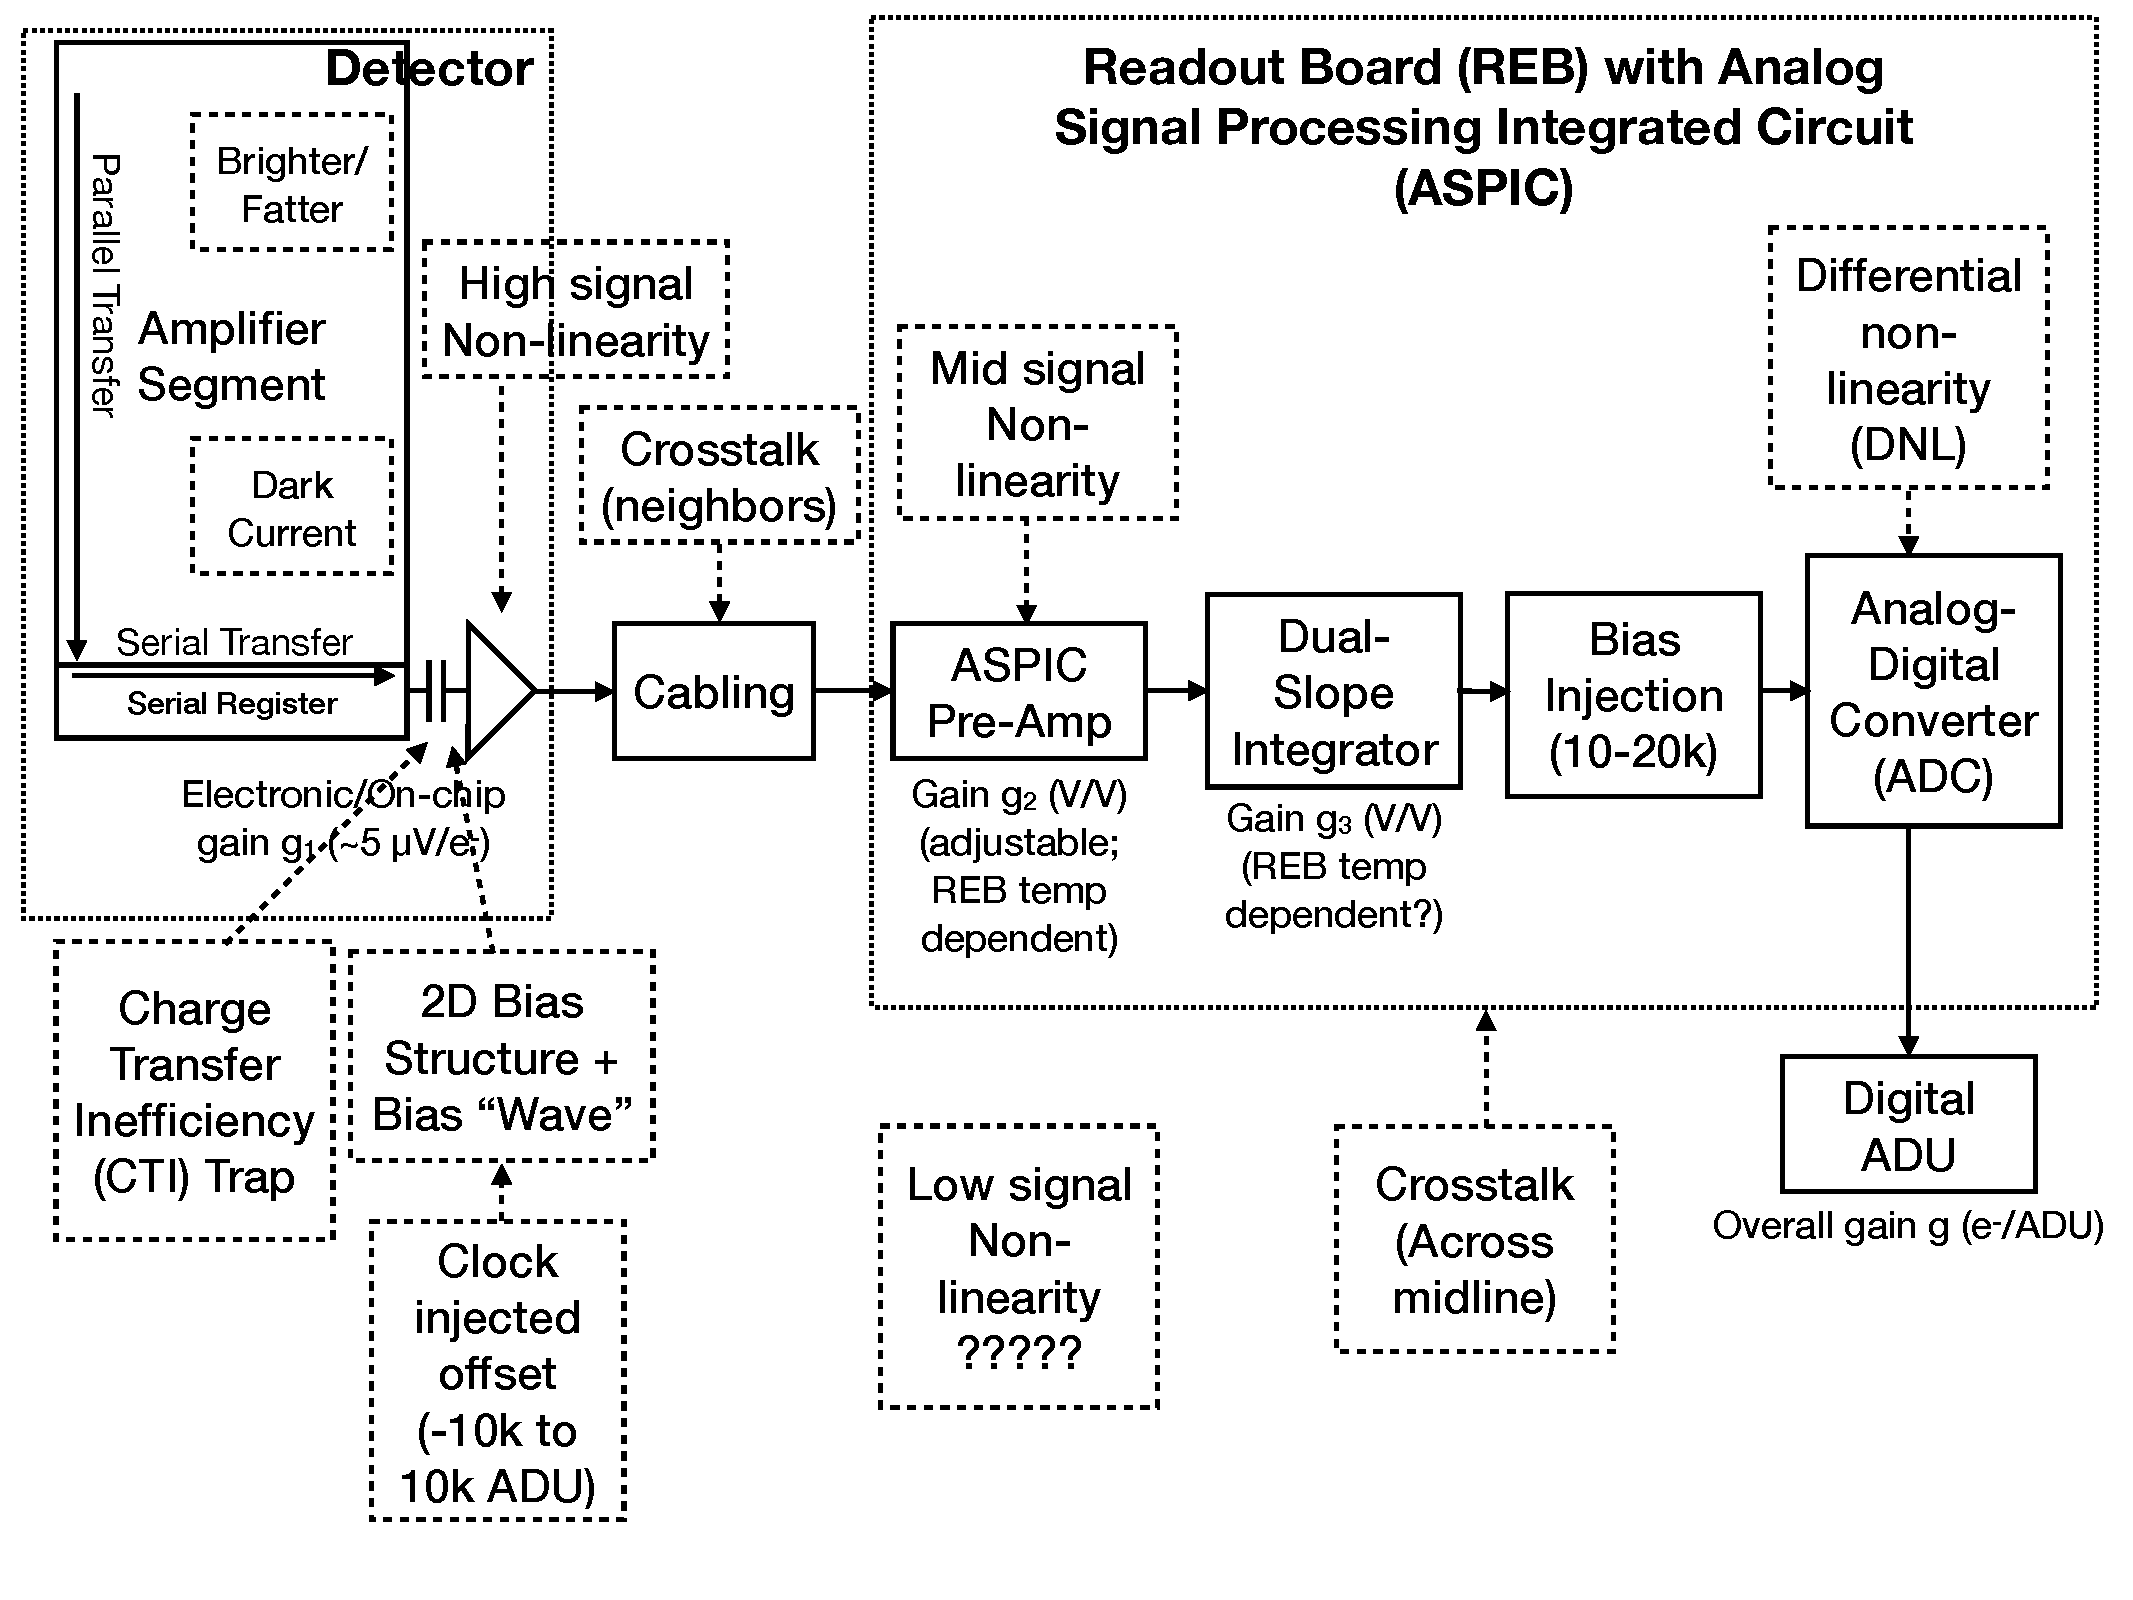
\includegraphics[width=0.98\linewidth]{drp/calibration_boxes_detector_model.pdf}
  \caption{The model of the detector and \gls{REB} components, labeled with the effects that they impart on signal.}
  \label{fig:isr_signal_chain}
\end{figure}

The \gls{ISR} processing pipeline for \gls{DP1} performs, in the following order: \gls{ADU} dithering to reduce quantization effects, serial overscan subtraction, saturation masking, gain normalization, crosstalk correction, parallel overscan subtraction, linearity correction, serial \gls{CTI} correction, image assembly, bias subtraction, dark subtraction, brighter-fatter correction, defect masking and interpolation, variance plane construction, flat fielding, and amplifier offset (amp-offset) correction\footnote{Amp-offset corrections are designed to address systematic discontinuities in background sky levels across amplifier boundaries. The implementation in the LSST Science Pipelines is based on the \texttt{Pan-STARRS} Pattern Continuity algorithm \citep{2020ApJS..251....4W}.}.
Flat fielding for \gls{DP1} was performed using combined flats produced from twilight flats acquired with sufficient rotational dithering to mitigate artifacts from print-through stars, as described in \secref{ssec:flat_field_system}.

% % Very detailed
% The following summarizes the ISR processing steps for DP1, in order of application.
% More details and a description of the full ISR processing envisaged for LSSTCam can be found at \citet{SITCOMTN-086}.
% \begin{description}
% \item[Dithering] Raw images are recorded in digitized ADU units, however the true input signal lies within a narrow range around the ADU value.
% Adding a random dither in the range [-0.5, 0.5) to each pixel reduces quantization-induced correlations in later corrections.
% This process introduces ~1/12 ADU to the image noise, which is negligible compared to other noise sources.

% \item[Serial Overscan Subtraction] After each row of pixels is read out, extra "overscan" pixels are recorded as the serial register continues clocking.
% We subtract the median value of each overscan row (excluding the first and last 3 columns) from the corresponding image row. This removes most of the electronic bias from the image.

% \item[Saturation Masking] Pixels with values above some threshold are excluded from further study, as they start to bleed charge into neighboring pixels.
%     Details on how this level is set are presented in \cite{SITCOMTN-086}.
%     DuringLSSTComCam commissioning, we noticed that very saturated sources created bleed trails that can extend to the edge of the detector in unique ways.
%     Examples of these trails are shown below in subsection \ref{ssec:sensor_anomalies}.
%     All saturated pixels, and the bleed features they can create, are added to the image mask to mark them either as saturated or bad, depending on the reason for being flagged.
%   \item[Gain Normalization] We determine the detector gains from the photon transfer curve method, and apply them to the images at this point.
%     This converts the pixel units from ADU to electrons, allowing the following corrections to operate in their natural units.
%     The images after gain normalization are significantly more consistent, as the gain differences account for most of the amplifier-to-amplifier offsets.
%   \item[Crosstalk Correction] A crosstalk correction subtrahend for a given ``target'' amplifier is generated by taking the images from all other amplifiers on that detector, flipped to ensure the ``source'' amplifier's readout corner matches the target, and then adding a copy scaled by the crosstalk coefficient from that source onto that target.
%     This is repeated for all amplifiers to build up a single image that is then subtracted from the input to remove the crosstalk signal.
%     As the crosstalk coefficients are small (the largest is approximately 3e-4), only the very brightest pixels on the source amplifier contribute significantly to this subtrahend image.
%     In addition, the crosstalk from distant amplifiers drops quickly, with non-neighbor crosstalk coefficients two to three orders of magnitude smaller.
%     Any pixel in the subtrahend image that is larger than 1 electron has the crosstalk bit set in the image mask, so the locations of such large corrections are available to downstream processing.
%     This correction is run over the entire image, including the parallel overscan region, to ensure that bright saturated star bleeds, which can extend into this region and crosstalk onto other amplifiers, are corrected.
%   \item[Parallel Overscan Subtraction] The parallel overscan is generated when the camera continues to shift data into the serial register after the image has been fully read out.
%     These additional rows see the same shifts in the bias level as the pixels are read out as the image region, and so can be used to remove this shift in the bias level from the image.
%     We again use a column-by-column median correction, which removes these bias shifts that change with time.
%   \item[Linearity Correction] We use a single spline-based linearity correction to account for all of the different sources of non-linearity throughout the signal chain.
%     This correction is applied at this point in the processing as it corresponds to the largest source of non-linearity, the output amplifier on the detector.
%   \item[Serial CTI Correction] The serial charge transfer inefficiency (CTI) is believed to be primarily created from the wiring connecting the serial register to the output amplifier.
%     Although the CTI is in general a small effect, one detector onLSSTComCam has a large measured correction, with a visible signature of amplifier edges that sag compared to the rest of the imaging region.
%     The correction reallocates the flux based on a model of charge traps and transfer efficiencies, and requires the serial overscan regions, as the inefficiently transferred flux is deposited into this region.
%   \item[Assembly] At this point in the processing, the image still contains all of the prescan and overscan regions, and so the data region is discontinuous.
%     This step trims these now-unnecessary regions, and merges the data regions from each amplifier into a single contiguous image.
%   \item[Bias Subtraction] Although most of the bias level has been removed from the overscan steps taken above, it is still possible that a static bias structure is present in each image.
%     By taking the clipped mean of a large number of zero-second exposures (with all of the ISR steps previously described), we can construct a ``combined bias'' that can be subtracted to remove the static signal still present from the bias.
%   \item[Dark Subtraction] In a similar fashion, we can construct a ``combined dark'' by using 30-second unilluminated exposures that tracks the dark current, which is the rate in electrons per second that pixels gain flux just by integrating.
%     This effect is small, and we mask any pixel with a dark current larger than 3 electrons per second as bad.
%   \item[Brighter-Fatter Correction] The brighter-fatter effect is a recently described phenomenon in which the size of an object increases as the accumulated charge in central pixels repel additional charges into neighboring pixels.
%     The correction for this attempts to restore the flux to where it should be, using a convolution process and the measured brighter-fatter kernel.
%     As this correction is non-local, it is sensitive to defects and detector edges, requiring the image to have defect pixels interpolated.
%     Correcting at the edge of the detector is not well defined, and so we mask pixels within one kernel size as ``EDGE''.

% \item[Defect Masking and Interpolation] A final cosmetic interpolation is done over all BAD and SAT pixel masks to ensure that visualizations and image scaling do not need to handle extreme values.
% As mentioned above, pixels with high dark current are part of our defect masks, and we also set pixels that are below 95\% of the median flat value as defects, as these pixels likely have poor quantum efficiency relative to their neighbors.

% \item[Variance Plane Construction] As we have converted the image back to units of electrons, we can set the variance plane as the sum in quadrature of the image itself (representing the Poissonian component) and the per-amplifier read noise values.

% After the above series of steps, we have an unflattened, gain normalized image with sensor
% effects removed.

% \item[Flat Fielding] Flat fielding for DP1 was performed using combined flats produced from twilight flats acquired with sufficient rotational dithering to mitigate artifacts from print-through stars, as described in \secref{ssec:flat_field_system}.

%\end{description}
